\pagebreak

\section{圆的基本概念}

\begin{definition}[圆的标准方程]
    因为能一眼看出圆的圆心和半径，所以圆的标准方程为 $(x-a)^2+(y-b)^2=r^2$，其中 $(a,b)$ 是圆心，$r$ 是半径。

    \begin{center}
        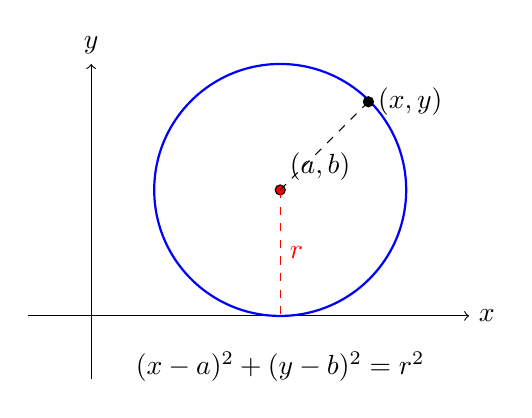
\begin{tikzpicture}[scale=0.8]
            % 绘制坐标轴
            \draw[->] (-1,0) -- (6,0) node[right] {$x$};
            \draw[->] (0,-1) -- (0,4) node[above] {$y$};

            % 绘制圆
            \draw[thick, blue] (3,2) circle (2);

            % 标记圆心和半径
            \draw[fill=red] (3,2) circle (0.08) node[above right] {$(a,b)$};
            \draw[dashed, red] (3,2) -- (3,0) node[midway, right] {$r$};

            % 标记一个圆上的点
            \draw[fill=black] (4.4,3.4) circle (0.08) node[right] {$(x,y)$};
            \draw[dashed] (3,2) -- (4.4,3.4);

            % 添加方程说明
            \node at (3,-0.8) {$(x-a)^2+(y-b)^2=r^2$};
        \end{tikzpicture}
    \end{center}
\end{definition}

\begin{definition}[圆的一般方程]
    圆的一般方程为 $x^2+y^2+Dx+Ey+F=0$，其中 $D$，$E$，$F$ 是常数。

    将一般方程变形为标准方程：
    \begin{align}
        x^2+y^2+Dx+Ey+F                                                       & = 0                              \\
        \left(x^2+Dx+\frac{D^2}{4}\right) + \left(y^2+Ey+\frac{E^2}{4}\right) & = -F+\frac{D^2}{4}+\frac{E^2}{4} \\
        \left(x+\frac{D}{2}\right)^2 + \left(y+\frac{E}{2}\right)^2           & = \frac{D^2+E^2-4F}{4}
    \end{align}

    因此，圆心坐标为 $\left(-\frac{D}{2}, -\frac{E}{2}\right)$，半径为 $r = \frac{\sqrt{D^2+E^2-4F}}{2}$。
\end{definition}

\begin{theorem}
    对于一般方程 $x^2+y^2+Dx+Ey+F=0$ 表示的图形：
    \begin{itemize}
        \item 当 $D^2+E^2-4F > 0$ 时，表示一个圆
        \item 当 $D^2+E^2-4F = 0$ 时，表示一个点
        \item 当 $D^2+E^2-4F < 0$ 时，不表示任何实数解的图形
    \end{itemize}
\end{theorem}